% Cover letter using letter.sty
\documentclass{letter} % Uses 10pt
%Use \documentstyle[newcent]{letter} for New Century Schoolbook postscript font
% the following commands control the margins:
\topmargin=-1in    % Make letterhead start about 1 inch from top of page 
\textheight=8in  % text height can be bigger for a longer letter
\oddsidemargin=0pt % leftmargin is 1 inch
\textwidth=6.5in   % textwidth of 6.5in leaves 1 inch for right margin
\usepackage[american]{babel}

\usepackage [autostyle, english = american]{csquotes}
\usepackage[version=3]{mhchem} 
\usepackage[hidelinks]{hyperref}
\usepackage{color}
\usepackage[ampersand]{easylist}
\usepackage{graphicx}
\usepackage{float}
\usepackage{caption}
\usepackage{amsmath}


\newfloat{figure}{htbp}{figs}

% \newcommand{\colornote}[1]{\textcolor{red}{ COMMENT\large\footnote{\textcolor{red}{#1}}}}
\newcommand{\colornote}[1]{\textcolor{red}{#1}}
\newcommand{\sci}[2]{ #1 \cdot 10^{#2}\ }
\newcommand{\pp}[1]{\left( #1\right)}


\begin{document}

\signature{Andrew S. Voyles}           % name for signature 
\longindentation=0pt                       % needed to get closing flush left
\let\raggedleft\raggedright                % needed to get date flush left
 
 
\begin{letter}{Mark Breese, PhD \\
Editor \\
Nuclear Instruments and Methods in Physics Research Section B: \\
Beam Interactions with Materials and Atoms}


\begin{flushleft}
{\large\bf Andrew S. Voyles}
\end{flushleft}
\medskip\hrule height 1pt
\begin{flushright}
\hfill The University of California, Berkeley \\
\hfill 1106B Etcheverry Hall, Berkeley, CA  94720-1730 \\
\hfill (850) 281-0217 or (510) 486-7310 
\end{flushright} 
\vfill % forces letterhead to top of page

 
\opening{Dear Dr. Breese,} 

  \renewcommand*{\thefootnote}{\alph{footnote}}

  \noindent I am writing to submit my point-by-point responses to the issues raised by the reviewers for my submitted manuscript entitled \enquote{\emph{Measurement of the \ce{^{64}Zn},\ce{^{47}Ti}(n,p) Cross Sections using a DD Neutron Generator for Medical Isotope Studies}}  for publication in Nuclear Instruments and Methods in Physics Research Section B.  Please find my responses detailed in \colornote{red text.}
  
  \noindent Along with my co-authors, I wanted to take the opportunity to personally thank you for your continued assistance in helping along the process of our submitted manuscript, and for finding such thorough and conscientious referees for reviewing it.  We would especially like to thank the referees for their thorough reading and critique, which has made it a better paper. All three were very constructive and pointed out many valuable improvements.
  
  Please find the feedback following here, and our revised manuscript attached. 
  
  Sincerely yours,\\ \\ \\ \\ Andrew S. Voyles
 
% \closing{Sincerely yours,} 

  \vfill
  
 \pagebreak
 
 
 
 Reviewer \#1:

describes the activation measurement of 64Zn(n,p)64Cu and 47Ti(n,p)47Sc with DD neutrons from the High-Flux Neutron Generator of University of California in Berkeley relative to indium (n,n') activation foils.
The produced radioactive isotopes 64Cu, 47Sc are relevant for nuclear medicine.
64Cu is a positron emitter, while 47Sc decays by beta-minus emission.
The use of DD neutrons has the advantage that at this energy no other radioactive copper or scandium isotopes are produced.

It features a very compact double sided titanium-copper target on which high intensity deuteron beams with 100 kV impinge from nearby ion sources from opposite sides.

In the experiment a deuteron current of 1.3 mA created a flux of 1.3E7 neutrons /cm2 /s on the target. Inside the target small activation samples can be mounted only 8 mm away from the neutron producing target surface. The target foils consisted of thin metallic zinc and titanium foils in
addition to indium foils to provide a reference for a relative measurement of the activation reactions by gamma-ray spectroscopy.

The neutron spectrum produced in the target is simulated with MCNP6 and an effective energy range for neutron activation of indium is determined.
The incident neutron energy also depends on the position of the deuteron beam spot on the target. A square array of nine indium foils  with smaller diameter is used to measure the neutron beam intensity. The beam seems mostly centered on the target;an asymmetry of the neutron beam intensity in the horizontal direction is illustrated in Fig. 8.

The induced activity of the irradiated zinc, titanium and indium samples is measured using HPGe detectors calibrated with several gamma-ray calibration sources. The half-live of the different indium and 64Cu activities are measured for a verification of the identification of the gamma-ray peaks.
The measured activity of the irradiated samples is used to determine the  cross section of 64Zn(n,p)64Cu and 47Ti(n,p)47Sc relative to 115In(n,n'). Statistical uncertainties due to the counting statistics are about 4 \%. The main systematic uncertainty is due to the uncertainty of the normalizing indium cross sections. Additional systematic uncertainties are the position
and size of the deuteron beam relative to the target irradiation samples as this induces a shift in the neutron energy spectrum of the activation. Additional uncertainties like the relative gamma-ray detection efficiency are not listed. The 115In neutron capture cross section was determined to
an effective energy of 2.45 MeV which indicates that there might be some contribution of lower energy neutrons contributing to the activation yield.

As several target positions can be irradiated simultaneously a group of activation cross sections from 2.6 to 2.7 MeV can be measured. The saturation activity that can be reached is proportional to activation cross section, the number of irradiated target atoms and the neutron flux per cm2 and second. This activity should be in the mCi range to be useful for
medical use. The quantity eta (eq.10) is added to the known formula for the activation by neutron irradiation as a dimensionless neutron utilisation factor.

The paper describes an activation cross section measurement with a
novel quasimonoenergetic neutron source using deuteron beams from two sides on a compact target assembly. It is well structured and nicely written and contains most aspects of the measurement. The neutron intensity of this source (at the future 1.E10 level might have the potential
to be useful for medical radioisotope production, although this point should be more clearly made in the discussion section.

The paper ist suitable for publication in NIM B after the following items have been addressed, which should be a minor revision. The corrections relate mainly to the fact, statements are made, but not quantified with numbers that should be easily available from the data analysis.

 \colornote{We would first like thank the reviewer for their extremely detailed summary and suggestions of the manuscript. It is clear that they read the manuscript thoroughly, and the feedback they have provided here has been vital for the improvement of the paper as a whole.}



\begin{easylist}[enumerate]
\ListProperties(Style2*=$\bullet~$,Numbers1=a,Hide2=100,FinalMark={)})
& The "neutron utilisation factor" eta is not clearly explained.
Usually "likelihood of a neutron inducing the desired reaction on one of the target sample atoms" is simply the cross section:  N$_{reac}$/ N$_{neutron}$ = sigma(Cm2) * n$_{target}$( atoms/cm2) To determine the saturation activity from an activation with a constant neutron flux this factor is not required.\\  The discussion of eq.(9) and (10) should be improved, and quantitative results related to the current measurement should be reported. Maybe eq.(10) is not required.\\
\textbullet\hspace{.1cm} \colornote{You are absolutely correct - we have reworked our discussion of the neutron utilization factor to clarify our intent, and link it to saturation activity.} \\ \\
The discussion section does not include the value of the saturation activity of the reported measurement, e.g. for 64Cu it should be ca. 1.5 kBq (using 1.3E7 n/(s cm2), 50 mbarn cross section and 0.5 g of nat-Zn). With some intensity improvements (factor 100-1000) which seems realistic, the mCi (37 MBq) range can be reached. This is however not stated in the
paper. \\
\textbullet\hspace{.1cm}\colornote{Thank you for pointing out this omission. Calculations for the theoretical saturation activities, as well as observed estimates of $\eta$ have now been added to the discussion in section 4 (see the third paragraph of P. 10).} 
& In an activation measurement the integral of the neutron spectrum and cross section determines the yield, see. eq.(1).
The thresholds for (n,p) on Cu or Ti and (n,n') on indium are not the same. Fig. 5 shows the effective energy range for indium only.\\ Is there systematic effect on the measured (n,p) cross sections due to the low energy tail of the neutron spectrum shown in Fig. 4 ?\\ 
\textbullet\hspace{.1cm} \colornote{We thank the referee for touching on an interesting point.  We believe that there is no shift in the magnitude of the cross section, since that is defined solely by the indium IRDFF value convolved with our flux. You are absolutely correct - the thresholds for (n,p) on Zn and Ti are not the same as for In.  
The difference in threshold causes the contribution to the activation due to energies below the main peak in the neutron energy spectrum, particularly the \enquote{low energy tail} near 2.25 MeV shown in figure 4, to be slightly different for the (n,p) reactions as compared to the (n,n') reaction. The only way to take into account this additional activation is by convolving the MCNP-modeled flux with the (n,p) cross sections from a model calculation.   This results in an additional systematic uncertainty in the width of our effective energy bin, since the modeled (n,p) cross sections are somewhat uncertain in this energy region.  \\ \\
Fortunately, the effect is quite modest.  The contribution to the $^{115m}$In activation in this energy region is 2.17\%.  The TALYS values for the production of $^{64}$Cu and $^{47}$Ti indicate that 0.24\% and 0.85\% of the activation can be attributed to the \enquote{low energy tail} near 2.25 MeV.   If we assume a $\pm$25\% uncertainty in the TAYLS cross sections for the two (n,p) reactions (meaning that the activation fraction could vary from 0.18\% to 0.30\% for the $^{64}$Cu and 0.637\% to 1.062\% for $^{47}$Sc), this would lead to a shift in the effective energy bin of 0.06\% and 0.21\%, respectively.  For the case of Sc, this would correspond to a systematic uncertainty of $\pm$5.7 keV, and $\pm$1.6 keV for $^{64}$Cu - these are within the precision of the current +10 keV/-20 keV effective energy bin, and can be considered negligible.
% Thank you for this comment.  You are absolutely correct - the thresholds for (n,p) on Zn and Ti are not the same as for In. Fig. 5 only shows the energy range in indium - a similar curve for (n,p) on Zn and Ti  would assume knowledge of a well-characterized low-energy excitation function for these, which does not currently exist, hence the motivation for this work. \\ \\The convolution of the IRDFF In(n,n') cross section with our MCNP neutron flux profile predicts that the total activity in the In produced by the low energy neutrons (below the \enquote{knee} near 2.25 MeV in  Fig. 4) is 2.17\%.  
% If we trust the (n,p) excitation functions for Zn and Ti from TALYS, the corresponding values from TALYS for the Cu and Sc activity are 0.24\% and 0.85\%, respectively.  
% If we assume an uncertainty of $\pm$100\% in the TALYS calculations in this energy region, the corresponding values from TALYS for the Cu and Sc activity are 0.47\% and 1.68\%, respectively. 
\\ \\ The low-energy tail in Figure 5 is not well-visible, due to Figure 5 being zoomed-in to illustrate how rapidly the $F(E')$ quantity rises over the 2.7-2.8 MeV range.  The zoomed-out version of this is seen below in  \autoref{fig:cu_xs_zoom}, which illustrates almost negligible contribution to the total activation until above 2.5 MeV neutrons.} \\ \\
The interpretation of the 115In capture cross section effective energy is not clear. \\ 
Can there be an estimate made on how many thermal neutrons are in the spectrum ?\\  
\textbullet\hspace{.1cm}\colornote{Based on MCNP, the thermal component  (0-0.0253 eV) makes up 0.00320\% of the total neutron population in the indium foils. Even considering epithermal neutrons (0-10 keV), they still only make up 0.0771\% of the total neutron population. The semilog axes of Fig. 4 exaggerate the relative population of thermal / epithermal neutrons. }\\ \\
What is the meaning of the data symbols in Fig. 4  and why does the spectrum stop at the
highest flux (around 4 units) should it not drop to zero yield above the 2.75 MeV peak ?\\
\textbullet\hspace{.1cm} \colornote{We have made changes to this figure in order to make it more readable -  thank you for the feedback to help improve it. Since the indium/activation foil spectra are so very similar to each other in Fig. 4 (and the voided/non-voided neutron production target spectra as well, above approx 2.6 MeV), the markers were added to differentiate the spectra if the manuscript were being viewed in greyscale / by a colorblind individual.  Without distinct  markers, the various spectra are nearly indistinguishable, due to the proximity of both target and indium foils to the DD reaction surface. \\ \\The peak flux occurs at 2.777 MeV - the 2.75 MeV number quoted on P. 3 was a typo and has been corrected. The flux does begin turning down above the peak, and the highest-energy neutron observed is at 2.783 MeV, as noted on P. 3 of the manuscript. Above 2.783 MeV, no neutrons are observed, but a value of y=0 cannot be plotted due to the log-y axes.  The drop to zero yield may be seen in a linear y-axis version of Fig. 4, seen in \autoref{fig:lin_xs_zoom} below. \\ \\These nuances and detailed information about the spectral shape (in particular the rapid rise above the 2.25 MeV shoulder) of the log-y version are masked in this lin-y version, which is why the former was chosen to be included in the manuscript.} 
& The HPGe and LEPS detectors were calibrated at various distances with calibration sources.
How well is the relative efficiency known for the gamma-rays used in the measurement ?
This could add to the systematic uncertainty. Especially 133Ba and 152Eu as multi-line sources might require a correction for coincident summing if the distance to the sample was small.
&& \colornote{Samples were counted far enough away (approx. 20 cm away, for a 1-cm diameter foil) to avoid any large coincident summing effects, and regardless, and ``no summing corrections needed to be made for the irradiated targets since all of the gammas are either non-coincident or formed in a back-to-back annihilation event'' (See P. 5, Line 1).  As for calibration, the relative efficiency of detectors is known to the 1-1.5\% level.  This efficiency uncertainty is included in the total uncertainty in section 2.6 (``With the exception of decay constants  and time measurement, which have negligible uncertainty compared to other sources of uncertainties in this work, each of the parameters in this model carries an uncertainty.''  (P. 8, lines 8-11))}
& In the description of the experiment it is never explicitely stated that deuteron beams were impinging from both sides on the target or not. Fig.1 seems to indicate that there are two deuteron ion sources, although Fig. 2 shows neutrons only coming from one side.
The authors should clarify the mode of operation.
&& \colornote{Thank you for the comments - this was an oversight and has been clarified, as only a single source was operated during this work.  This has been clarified on page 1, end of section 2.1 (``While the machine's design\ldots'').}
\end{easylist}

\begin{figure}
 \centering
 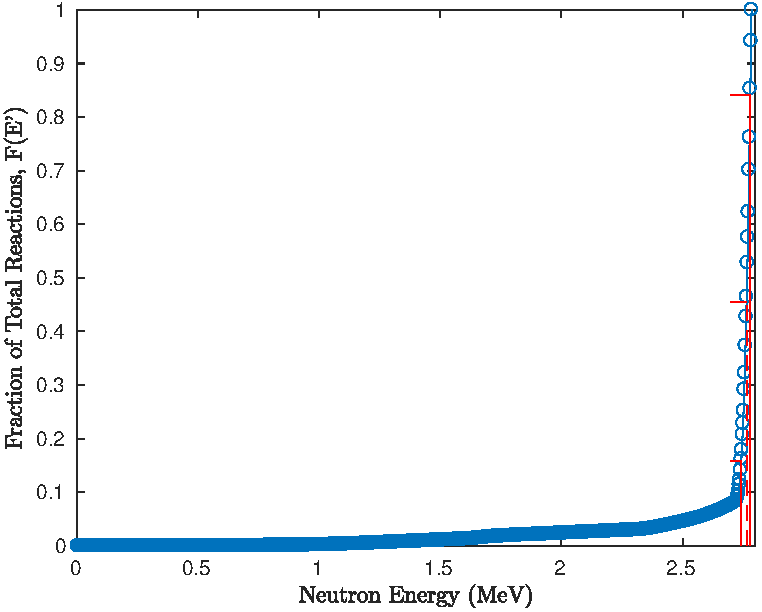
\includegraphics[scale=0.65]{./figures/zoomed_out_fracplot.pdf}
 % zoomed_out_fracplot.pdf: 366x294 pixel, 72dpi, 12.91x10.37 cm, bb=0 0 366 294
 \caption{Zoomed-out version of Figure 5 from the manuscript.}
 \label{fig:cu_xs_zoom}
\end{figure}

\begin{figure}
 \centering
 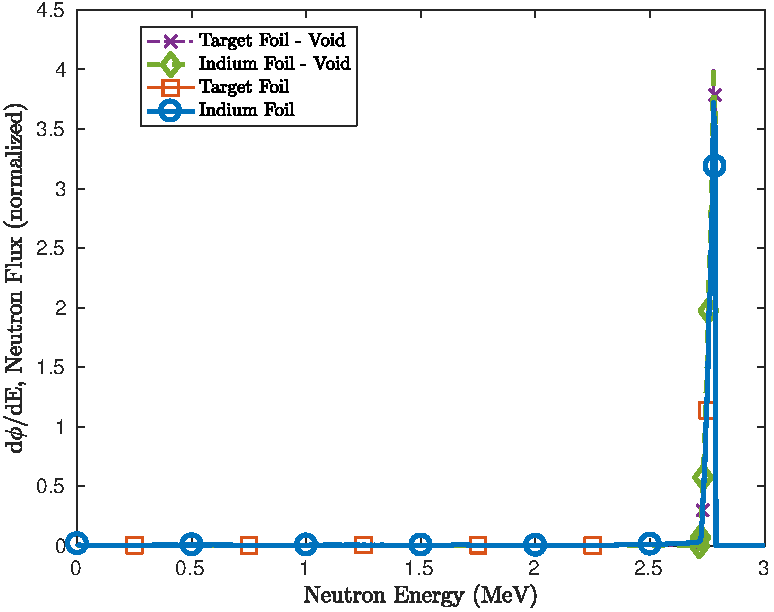
\includegraphics[scale=0.65]{./figures/lin_mcnp_flux.pdf}
 % zoomed_out_fracplot.pdf: 366x294 pixel, 72dpi, 12.91x10.37 cm, bb=0 0 366 294
 \caption{Linear y-axis version of Figure 4 from the manuscript.}
 \label{fig:lin_xs_zoom}
\end{figure}

Typos:

\begin{easylist}[enumerate]
\ListProperties(Style2*=$\bullet~$,Numbers1=a,Hide2=100,FinalMark={)})
& p.1 line 45 right column "their energy spectra are often not well-suited"
&& \colornote{Typo corrected.}
& p.2 line 27 left: 47Sc is not a positron emitter
&& \colornote{Roles of each radionuclide have been clarified.}
& p.10. line 31 Ref.[1] is incomplete.
&& \colornote{Reference updated.  See the Reviewer \#2 section for more detail.}
\end{easylist}

 \pagebreak
 
 %\\ The 115In capture note is more of an observation than a reportable. The cross sections we have measured are for the effective neutron energy of 2.76 MeV. At this energy, the 116In activity produced would predict a 64Zn(n,p)64Cu cross section, for example, of approx 41 mb, which is approx 20\% lower than the cross sections relative to the 113mIn and 115mIn standards. This is because the 116In capture activity is far more sensitive to lower-energy neutron contributions than the 113mIn/115mIn inelastic scattering activities. As a simple exercise, one can very the effective neutron energy for the 116In capture channel until the 64Zn(n,p)64Cu cross section observed (relative to the 116In ``monitor channel'') agrees with the 113mIn/115mIn monitor channels.  This occurs if one assumes an effective neutron energy of 2.45 MeV for 115In(n,gamma)116In.  The point we were making in describing this observation is that it offers further proof that there are very few thermal neutrons seen by the target positions in the HFNG - otherwise, the effective neutron energy would have shifted far lower in energy than from 2.76 MeV to just 2.45 MeV.  This low population of thermals, in turn, confirms that DD neutrons are a potentially effective method to produce radionuclides with high specific activity (very little unwanted competing nuclides produced) - the low energy of DD neutrons energetically prevents (n,pn) channels from being open for production, and the apparent tiny population of thermal/epithermal neutrons makes (n,gamma) contamination minimal, relative to the desired (n,p) channel.
 %The peak flux occurs at 2.777 MeV - the 2.75 MeV number quoted on P. 3 was a typo and has been corrected. However, the energy of the peak flux is expected to be higher than the flux-weighted average of 2.765 MeV, as the low-energy contributions shift the flux-weighted average down in energy. However, the tiny shift below the peak is further evidence of how few thermal / low-energy neutrons are present. As for the zero yield, yes, the flux does begin turning down above the peak, and the highest-energy neutron observed is at 2.783 MeV, as noted on P. 3 of the manuscript. Above 2.783 MeV, no neutrons are observed. However, in plotting on log axes, a value in $y$ of 0 cannot be plotted, as ln(0) is undefined.  This is why the curve appears to stop instead of immediately dropping to zero, and the drop to zero yield may be seen in a linear y-axis version of Fig. 4, seen in \autoref{fig:lin_xs_zoom} below. This nuances and detailed information about the spectral shape (in particular the rapid rise above the 2.25 MeV shoulder) of the log-y version are masked in this lin-y version, which is why the former was chosen to be included in the manuscript.

Reviewer \#2:

 This article describes the use of a modern, compact D-D neutron source to produce radioisotopes for medical and other applications. The radioisotopes 47Sc and 64Cu were chosen because they have potential for diagnostic or therapeutic medical applications, and can be produced using the (n,p) reaction that is an open reaction channel at the energy of the neutron source. The radioisotope production cross sections were measured relative to indium inelastic activation cross sections that are well determined. The authors performed a thorough and detailed analysis of the energy and angle dependence of the neutron flux, as well as properly accounting for the production and decay of the radioisotopes in determining the reaction cross sections. The resulting cross section values agree within uncertainties with some previous measurements and have smaller uncertainties than previous work. The results show the potential of using such a compact D-D neutron source for both medical
radioisotope production and nuclear research. Because the work is of interest to the NIM B audience, is thorough and well-presented, it should be published. There are however, some minor corrections to the text that are necessary, as well as some changes to the references that are needed before publication. These corrections are listed below.

\colornote{We would first like thank the reviewer for their very thoughtful and helpful suggestions of the manuscript. The feedback they have provided here has been extremely helpful for correcting a number of outstanding typos and improvements for the references cited.}


\begin{easylist}[enumerate]
\ListProperties(Style2*=$\bullet~$,Numbers1=a,Hide2=100,FinalMark={)})
& P 1 "energy spectra is…" should be "energy spectra are…"

&& \colornote{Typo corrected.}
& P 2 "100 kV deuterium beam" correct "kV" to "keV"

&& \colornote{Typo corrected.}
& P 4 Table 1. My preference is for "at. \%" rather than "a/o"

&& \colornote{Change implemented.}
& P 5 missing "to" in "subjected to this flux" and Fig. 8 - the authors should comment on the significance of the flux at right (8.35 E6) that is nearly the same as the center value.


&& \colornote{Change implemented.  In addition, more discussion of the small horizontal asymmetry in neutron flux is provided in the same paragraph.}
& P 8 "makes indium a better" correct to "make indium …"; "for incident" should be "for an incident"; and "The results for the production of 116In …" should be "The result…".


&& \colornote{Changes implemented.}
\end{easylist}

References -


\begin{easylist}[enumerate]
\ListProperties(Style2*=$\bullet~$,Numbers1=a,Hide2=100,FinalMark={)})
& [1] - this reference needs details of the source - report, book or article and particulars

&& \colornote{Reference Updated.  The report is only publicly available from\\ \url{https://www.aaas.org/report/nuclear-medicine-without-nuclear-reactors-or-uranium-enrichment}, but the reference has been updated with more detail.}
& [2] - page and year of journal article are needed

&& \colornote{Article was accepted and in publication at the time of this manuscript's submission, but has now been published.  Reference updated.}
& [3] - a URL for access to the dissertation would benefit the reader

&& \colornote{The Elsevier-recommended \url{elsarticle-num} BibTeX style does not support a URL in a PhD Thesis citation. I have hacked one in, \emph{but the editors are welcome to remove it in the final processing if it does not conform to journal style standards.} If another method for referencing a URL is preferred, the Thesis is hosted by UC Berkeley at  \url{http://search.proquest.com/docview/1834600459}}
& Along with references 2 and 3, adding Q. Ji, A. Sy, and J. W. Kwan, Rev. Sci. Instr. 81, 02B312 (2010) is needed for completeness.

&& \colornote{Per Ref [2,3], the ion sources used in the HFNG are based on the similar design of the Ji (2010) article, but not identical. This has been noted on p.2 lines 12-13, right column (``using ion sources\ldots'') . }
& [13] - page and year are needed

&& \colornote{Reference updated.}
& [25] Add "Los Alamos Report" LA-UR-13-22934

&& \colornote{Reference updated.}
& [30] Add URL - http://radware.phy.ornl.gov/gf3/gf3.html

&& \colornote{See above.  URLs are not allowed in this BibTeX format; I hacked it in, but the editors are welcome to remove it in order to maintain journal style.}
\end{easylist}

 \pagebreak



Reviewer \#3:

Excellent contribution to the field of medical radioisotope production.
I believe there is one significant omission from the discussion.
What do the authors believe will be the attainable saturation activity for the two nuclides considered?

The principle of the estimate is indicated. The numbers are missing. These numbers should be compared with foreseen need.

\colornote{We would first like thank the reviewer for their very favorable impression of our manuscript.  They pointed out a significant omission preventing the work from cohesively tying  together the science herein and the application space it seeks to serve.}

\begin{easylist}[enumerate]
\ListProperties(Style2*=$\bullet~$,Numbers1=a,Hide=2,FinalMark={)})
& 

&& \colornote{Theoretical saturation activities (based on operating conditions at the time of the work in this manuscript) have been added to section 4 (see the first paragraph of P. 10).  In addition, brief discussion of the steps necessary to increase the saturation activity to the mCi level are suggested.}
\end{easylist}

% \pagebreak


 

 
% \encl{}  				% Enclosures

\end{letter}
 

\end{document}